\chapter{Opérations sur les nombres décimaux}\label{ChOpNombresDecimaux}

\vspace{5cm}
\begin{acquis}
\begin{itemize}
\item Savoir effectuer une succession d'opérations avec ou sans parenthèses, en respectant les règles de priorité et sans calculatrice.
\item Savoir donner une valeur approchée d'un nombre relatif (par excès, par défaut et troncature).
\columnbreak
\item Savoir résoudre des problèmes utilisant les 4 opérations, en n'utilisant qu'une seule expression mathématique.
\end{itemize}
\end{acquis}


%\activites  % pas d'activité dans ce chapitre
%\input{OpNombresDecimaux/OpNbDec_acti.tex}

\cours
\section{Rappels sur les opérations avec des nombres relatifs}

\subsection{Addition / soustraction de nombres relatifs}

\begin{rappel}
La \MotDefinition{valeur absolue}{} d'un nombre relatif est \textbf{le nombre sans son signe}. Sur une droite graduée, cela correspond à la distance entre l'origine et le point qui a pour abscisse ce nombre.
\end{rappel}


\begin{aconnaitre}
Pour \textbf{additionner deux nombres relatifs de même signe}, on additionne leur valeur absolue et on garde le signe commun.

Pour \textbf{additionner deux nombres relatifs de signes contraires}, on soustrait la plus petite valeur absolue de la plus grande et on prend le signe de celui qui a la plus grande valeur absolue.

\textbf{Soustraire un nombre relatif} revient à ajouter \textbf{son opposé} (\textbf{L'opposé d'un nombre relatif} est le nombre de signe contraire qui a la même valeur absolue).
\end{aconnaitre}


\begin{exemple*1}
Effectue l'addition suivante : $A = (-2) +(-3)$. 

\correction

\begin{tabular}{lcl}
$A = (-2) +(-3)$ & $\rightarrow$ & On veut additionner deux nombres relatifs de même signe. \\
$A = -(2 +3)$ & $\rightarrow$ & On additionne leur valeur absolue et on garde le signe commun : $-$. \\
$A = -5 $ & $\rightarrow$ &  On calcule. \\
\end{tabular}

\end{exemple*1}





\begin{exemple*1}
Effectue l'addition suivante : $B = (-5) +(+7)$.  

\correction

\begin{tabular}{lcl}
$B = (-5) +(+7)$ & $\rightarrow$ & On veut additionner deux nombres relatifs de signes contraires. \\
$B = +(7 -5)$ & $\rightarrow$ & On soustrait leur valeur absolue et on écrit le signe du nombre qui a \\
& & la plus grande valeur absolue $(+7)$. \\
$B = +2$ & $\rightarrow$ & On calcule. \\
\end{tabular}

\end{exemple*1}





\begin{exemple*1}
Effectue la soustraction suivante : $C = (-2) -(-3)$. 

\correction

\begin{tabular}{lcl}
$C = (-2) -(-3)$ & $\rightarrow$ &  On veut soustraire le nombre $-3$\\
$C = (-2) +(+3)$ & $\rightarrow$ &  On ajoute l'opposé de $-3$ qui est $+3$.\\
$C = +(3 -2)$ & $\rightarrow$ &  On ajoute deux nombres de signes contraires donc on soustrait \\
& & leur valeur absolue et on prend le signe du nombre qui a la plus \\
& & grande valeur absolue $(+3)$. \\
$C = +1$ & $\rightarrow$ &  On calcule.\\
\end{tabular}

\end{exemple*1}
 



\subsection{Multiplication / division de deux nombres relatifs}

\begin{aconnaitre}
Pour multiplier (ou diviser) deux nombres relatifs, on multiplie (ou on divise) leur valeur absolue et on applique la \MotDefinition{règle des signes}{} suivante :
\begin{itemize}
    \item le produit de deux nombres relatifs de \textbf{même signe} est \textbf{positif} ($"+" \times "+" = "+"$ et $"-" \times "-" = "+"$) ;
    \item le produit de deux nombres relatifs de \textbf{signes contraires} est \textbf{négatif} ($"+" \times "-" = "-"$ et $"-" \times "+" = "-"$).
\end{itemize}
\end{aconnaitre}	





\begin{exemple*1}
Effectue la multiplication : $F = (-4) \times (-2,5)$.

\correction
Le résultat est positif car c'est le produit de deux nombres relatifs de même signe (négatifs).

$F = 4 \times 2,5 \qquad F = 10$
\end{exemple*1}

\begin{exemple*1}
Effectue la division : $G = 6,8 \div (-2)$.

\correction
Le résultat est négatif car c'est le quotient de deux nombres de signes contraires (un nombre positif par un nombre négatif).

$G = -(6,8 \div 2) \qquad		G = -3,4$
\end{exemple*1}

\begin{remarque}
Multiplier un nombre relatif par $-1$ revient à prendre son opposé.
\end{remarque}


\subsection{Multiplication de plusieurs nombres relatifs}

\begin{aconnaitre}
Le produit de plusieurs nombres relatifs est : 
\begin{itemize}
    \item \textbf{positif} s'il comporte un nombre \textbf{pair} de \textbf{facteurs négatifs};
    \item \textbf{négatif} s'il comporte un nombre \textbf{impair} de \textbf{facteurs négatifs}.
\end{itemize}
\end{aconnaitre}

\begin{exemple*1}
Quel est le signe du produit : $H = -6 \times 7 \times (-8) \times (-9)$ ?

\correction
Le produit comporte trois facteurs négatifs. Or 3 est impair donc $H$ est négatif.
\end{exemple*1}


\begin{exemple*1}
Calcule le produit : $J = 2 \times (-4) \times (-5) \times (-2,5) \times (-0,8)$.

\correction
Le produit comporte quatre facteurs négatifs. Or 4 est pair donc $J$ est positif.
$J = 2 \times 4 \times 5 \times 2,5 \times 0,8$

$J = (2 \times 5) \times (4 \times 2,5) \times 0,8$

$J = 10 \times 10 \times 0,8 = 80 $
\end{exemple*1}


\section{Priorité des opérations}

\begin{aconnaitre}
Dans une suite d'opérations avec des nombres relatifs, on effectue \textbf{dans l'ordre} : d'abord les calculs entre parenthèses puis les calculs de puissances, les multiplications et divisions et enfin les additions et soustractions.
\end{aconnaitre}


\begin{exemple*1}
Effectue le calcul suivant : $M = -4 -5 \times (-2 -6)$.

\correction

\begin{tabular}{lcl}
$M = -4 -5 \times \underline{(-2 -6)}$ & $\rightarrow$ & On repère le calcul prioritaire. \\
$M = -4 \underline{-5 \times (-8)}$ & $\rightarrow$ & On effectue d'abord le calcul entre parenthèses. \\
$M = \underline{-4 + 40}$ & $\rightarrow$ & On effectue ensuite la multiplication. \\
$M = 36$ & $\rightarrow$ & On termine par l'addition. \\
\end{tabular}
\end{exemple*1}





\section{Approximation de nombres relatifs}

\subsection{Troncature}

\begin{definition}
Prendre la troncature d’un nombre à une précision donnée, c’est couper ce nombre et enlever tous les chiffres qui dépassent la précision demandée.
\end{definition}

\begin{exemple*1}
Donner la troncature à $10^{-2}$ de $349,7275$ et la troncature au dixième de $57,93$.
\correction
La troncature à $10^{-2}$ de $349,7275$ est $349,72$ et la troncature au dixième de $57,93$ est $57,9$.
\end{exemple*1}

\subsection{Valeur approchée par défaut et par excès}
 
\begin{remarque}
Lorsqu’un nombre comporte plusieurs chiffres après la virgule, on peut en donner une valeur approchée à :
$10^{-1}$ près, c’est-à-dire 1 chiffre après la virgule. C’est une valeur approchée au dixième.
$10^{-2}$ près, c’est-à-dire 2 chiffres après la virgule. C’est une valeur approchée au centième.
$10^{-3}$ près, c’est-à-dire 3 chiffres après la virgule. C’est une valeur approchée au millième.
\end{remarque}

\begin{definition}
La \MotDefinition{valeur approchée à l’unité par défaut}{} d’un nombre est le nombre entier immédiatement plus petit que notre nombre.

La \MotDefinition{valeur approchée à l’unité par excès}{} d’un nombre est le nombre entier immédiatement plus grand que notre nombre.
\end{definition}

\begin{exemple*1}
Donner les valeurs approchées par défaut et par excès, à l'unité, du nombre $12,58$.

\correction
Le nombre entier immédiatement plus petit que $12,58$ est $12$. Donc la valeur approchée par défaut à l'unité de $12,58$ est $12$. Le nombre entier immédiatement plus grand que $12,58$ est $13$. Donc la valeur approchée par excès à l'unité de $12,58$ est $13$.
\end{exemple*1}



\begin{definition}
La \MotDefinition{valeur approchée au dixième par défaut}{} d’un nombre est le nombre décimal ayant un seul chiffre après la virgule immédiatement plus petit que notre nombre.

La \textbf{valeur approchée au dixième par excès}{} d’un nombre est le nombre décimal ayant un seul chiffre après la virgule immédiatement plus grand que notre nombre.
\end{definition}

\begin{exemple*1}
Donner les valeurs approchées par défaut et par excès au dixième du nombre $8,193$.

\correction
Le nombre ayant un chiffre après la virgule et qui est immédiatement plus petit que $8,193$ est $8,1$. Donc la valeur approchée par défaut au dixième (ou à $10^{-1}$) de $8,193$ est $8,1$. Le nombre ayant un chiffre après la virgule et qui est immédiatement plus grand que $8,193$ est $8,2$. Donc la valeur approchée par excès au dixième (ou à $10^{-1}$) de $8,193$ est $8,2$.
\end{exemple*1}


\begin{remarque}
On définit de la même façon la valeur approchée par défaut ou par excès à une précision donnée : valeur approchée par défaut à 10-2 près (au centième), ou valeur approchée par excès à 10-4 près (au dix-millièmes) ...
\end{remarque}


\subsection{Arrondi}

\begin{definition}
Donner l’arrondi d’un nombre positif, c’est déterminer \textbf{une valeur approchée de ce nombre en fonction du chiffre qui suit directement sa troncature} :
\begin{itemize}
    \item Si ce chiffre est 0, 1, 2, 3 ou 4, l’arrondi correspond à la troncature.
    \item Si ce chiffre est 5, 6, 7, 8 ou 9, on rajoute 1 au dernier chiffre de sa troncature.
\end{itemize}
\end{definition}

\begin{exemple*1}
Donner les arrondis à $10^{-2}$ et $10^{-3}$ de $83,372851$. Donner la troncature au dixième et l’arrondi au dixième de $175,378$.
\correction
L'arrondi à $10^{-2}$ de $83,374851$ est $83,37$ (car le chiffre des millièmes est 4) et l'arrondi à $10^{-3}$ est $83,375$ (car le chiffre des dix-millièmes est 8).

La troncature au dixième de $175,378$ est $175,3$ et l’arrondi au dixième est $175,4$ (car le chiffre des centièmes est 7).
\end{exemple*1}


\exercicesbase
\begin{colonne*exercice}

\serie{Additionner et soustraire}


\begin{exercice}Effectue les additions suivantes :
\begin{enumerate}
\item $(+4) +(+9)$
\item $(-2) +(+3)$
\item $(-4) +(-11)$
\item $(+1) +(-7)$
\item $(-10) +(+10)$
\item $(-40) +(+20)$
\end{enumerate}
\end{exercice}


\begin{exercice}Effectue les calculs suivants :
\begin{enumerate}
\item $9 -12$
\item $-10 -6$
\item $-2 - (-17)$
\item $-13 - (-5)$
\item $8 -1$
\item $0 -(-72)$
\end{enumerate}
\end{exercice}


\begin{exercice}Effectue les calculs suivants :
\begin{enumerate}
\item $15,7 +22,8$
\item $-51,5 +31,7$
\item $7,2 -3,1$
\item $31,2 -13,4$
\item $-2,8	- (-3,9)$
\item $-50	-12,4$
\end{enumerate}
\end{exercice}


\begin{exercice}Effectue les calculs suivants :
\begin{enumerate}
\item $5 -17$
\item $8 -21$
\item $-5 -2$
\item $-7 +11$
\item $31 -37$
\item $-2,8 -2,1$
\item $-8,3 +3,5$
\item $1,7 -3,52$
\end{enumerate}
\end{exercice}


\begin{exercice}Effectue les calculs suivants :
\begin{enumerate}
\item $13,2 +12,8$
\item $-25,5 +11,7$
\item $2,3 +(-1,5)$
\item $17,4 - (12,6)$
\item $-3,9 - (-11,1)$
\item $-100 - (+13)$
\end{enumerate}
\end{exercice}


\columnbreak
\begin{exercice}Effectue les calculs suivants (tu peux  regrouper les termes de même signe) :

$A = 24 +8 -12 +1 -5$

$B = -14 +5 -7 -10 +13$

$C = 11 -(-5) +(-8) +1 -(+17)$

$D = -11 -(+4) +23 +(-12) -(-18)$
\end{exercice}


\begin{exercice}Effectue les calculs suivants (tu peux  regrouper les termes de même signe) :

$A = 15 +3 -6 +2 -7 $

$B = -8 +4 -5 -6 +11$

$C = 10 -(-4) +(-1) +5 -9$

$D = (-15) -(+14) +30 +(-15) -(-20)$
\end{exercice}


\begin{exercice}Regroupe les termes astucieusement puis calcule :

$A = 22 +25 +8 -25$

$B = -1,5 +5,7 -3,6 +0,3 +1,5$
\end{exercice} 



\serie{Multiplier}



\begin{exercice}Calcule mentalement :
\begin{enumerate} 
\item $(-8) \times (+2)$
\item $(-2) \times (+5)$
\item $(-4) \times (-8)$
\item $(+9) \times (+10)$
\item $(+191) \times (+0,1)$ 
\item $(-1,5) \times (+20)$
\item $(-0,25) \times (-4)$
\item $(+0,8) \times (-3)$
\item $(-3,2) \times (+4)$
\item $(-1) \times (-17)$
\end{enumerate}
\end{exercice}



\begin{exercice}Relie chaque calcul à son résultat :
\begin{colitemize}{2}
\item $(+5) \times (-7)$
\item $(-6) \times (-4)$
\item $(-4) \times (+3)$
\item $(+7)	\times (+7)$
\item $(-3) \times (-4)$
\item $(-9) \times (-3)$
\item $(-5) \times (+3)$
\item $(-8) \times (+6)$
\item $-15$
\item $-35$
\item $-12$
\item $+12$
\item $-48$
\item $+27$
\item $+24$
\item $+49$
\end{colitemize}
\end{exercice}



\begin{exercice}Calcule, sachant que $11,2 \times 2,5 = 28$ :
\begin{enumerate}
\item $11,2 \times (-2,5)$
\item $-11,2 \times (-2,5)$
\end{enumerate}
\end{exercice}


\newpage
\begin{exercice}[Un produit peut en cacher un autre...]
\begin{enumerate}
\item Calcule le produit $7,5 \times 0,2$.
\item Effectue alors les calculs suivants :
\subitem $A = 7,5 \times (-0,2)$
\subitem $B = (-0,2) \times (-7,5)$
\subitem $C = (-75) \times (+0,2)$
\subitem $D = (-7,5) \times (-20)$
\end{enumerate}
\end{exercice}



\begin{exercice}Complète les « pyramides » suivantes sachant que le nombre contenu dans une case est le produit des nombres contenus dans les deux cases situées en dessous de lui :
\end{exercice}


\begin{exercice}Effectue les calculs suivants :

$A = (-4) \times (-7) \times (+5)$

$B = (-2) \times (-5) \times (-3)$

$C = (+5) \times (-1) \times (+9)$
\end{exercice}



\begin{exercice}Effectue les calculs suivants :

$A = (-2,2) \times (-10) \times (+3) \times (-0,5)$

$B = (-50) \times (-0,25) \times (+4) \times (+2)$

$C = (-4) \times (-0,1) \times (+5) \times (+4)$

$D = (-1,5) \times (+4) \times (-1) \times (+0,8) \times (-3)$

$E = (+4) \times (-10) \times (+2) \times (-1) \times (-1)$
\end{exercice}



\begin{exercice}Calcule astucieusement :

$A = (-2) \times (-1,25) \times (-2,5) \times (-8)$

$B = (-75) \times (-0,25) \times (+2) \times (+4)$

$C = (+0,01) \times (-25) \times (-13) \times 4 \times (-3)$
\end{exercice}



\begin{exercice}Calcule dans chaque cas le produit $xy$ :
\begin{enumerate}
\item $x = 5 et y = -3$
\item $x = +4 et y = -11$
\item $x = -2 et y = -5$
\item $x = -0,5 et y = -5,2$
\end{enumerate}
\end{exercice}



\begin{exercice}Complète le tableau suivant :

\renewcommand*\tabularxcolumn[1]{>{\centering\arraybackslash}m{#1}}
\renewcommand{\arraystretch}{1.6}
\begin{ltableau}{\linewidth}{6}
\hline
$a$ & $b$ & $c$ & $ab$ &  $-(ac)$ & $abc$ \\ \hline 
$-5$ & 6 & $-4$ & & &  \\ \hline
$-1$ & $-2$ & $-3$ &  & & \\ \hline
$-2,1$ & $-4$ & $+3$  & & & \\ \hline
\end{ltableau}
\end{exercice}


\columnbreak
\begin{exercice}[Décompositions...]
\begin{enumerate}
\item Trouve toutes les façons de décomposer le nombre $-20$ en produit de deux nombres entiers relatifs.
\item Trouve toutes les façons de décomposer le nombre 24 en produit de trois nombres entiers relatifs.
\end{enumerate}
\end{exercice} 



\serie{Diviser}



\begin{exercice}Calcule mentalement :
\begin{enumerate}
\item $64 \div (-4)$
\item $48 \div (-8)$
\item $-27 \div (-3)$
\item $72 \div (+9)$
\item $-71 \div ( -1)$
\item $-42 \div 7$
\item $(-42) \div (-6)$
\item $125 \div (-5)$
\item $(-7) \div (+7)$
\item $(-29) \div (+1)$
\end{enumerate}
\end{exercice}



\begin{exercice}Calcule mentalement :
\begin{enumerate}
\item $(-100) \div (+25)$
\item $(-42) \div (-4)$
\item $(+54) \div (-3)$
\item $(+55) \div (+5)$
\item $(-24) \div (-5)$
\item $(-13) \div (-10)$
\end{enumerate}
\end{exercice}


\begin{exercice}Pour chaque fraction, trouve l'écriture la plus simple possible : 

Exemple : $\dfrac{-2}{+9}=-\dfrac{2}{9}$
\begin{enumerate}
\item $-\dfrac{+4}{+5}$
\item $-\dfrac{-1}{-5}$
\item $\dfrac{7}{-3}$
\item $-\dfrac{-8}{11}$
\item $-\dfrac{1}{-10}$
\item $-\dfrac{5}{-15}$
\end{enumerate}
\end{exercice}


\newpage
\begin{exercice}Sans calculatrice, donne l'écriture décimale de chacun des nombres suivants :
\begin{enumerate}
\item $-\dfrac{3}{-10}$
\item $-\dfrac{-64}{-8}$
\item $\dfrac{-50}{+100}$
\item $\dfrac{-3}{-2}$
\end{enumerate}
\end{exercice}



\begin{exercice}Utilise ta calculatrice pour donner l'écriture décimale des nombres suivants :
\begin{enumerate}
\item $\dfrac{-5}{-40}$
\item $-\dfrac{172}{-5}$
\item $-\dfrac{-125}{-625}$
\item $\dfrac{-0,235}{+0,8}$
\end{enumerate}
\end{exercice}



\begin{exercice}Dans chaque cas, calcule le quotient de $x$ par $y $:
\begin{enumerate}
\item $x = -15$ et $y = -3$
\item $x = +64$ et $y = -8$
\item $x = -36$ et $y = 12$
\item $x = -2,4$ et $y = 1,2$
\item $x = y = -2,3$
\item $x = 0$ et $y = -5$
\end{enumerate}
\end{exercice}



\begin{exercice}Complète le tableau suivant et donne le résultat sous forme décimale :

\renewcommand*\tabularxcolumn[1]{>{\centering\arraybackslash}m{#1}}
\renewcommand{\arraystretch}{1.6}
\begin{ltableau}{\linewidth}{6}
\hline
$a$ & $b$ & $c$ & $a \div b$ &  $-(b) \div c$ & $c \div (-a)$ \\ \hline 
$-5$ & 4 & $-4$ & & &  \\ \hline
$-2,5$ & $-1$ & $+20$ &  & & \\ \hline
$+8$ & $-4$ & $-0,5$  & & & \\ \hline
$-2,4$ & $-1,2$ & $-24$  & & & \\ \hline
\end{ltableau}
\end{exercice} 



\serie{Calculs variés}



\begin{exercice}Pour chacun des calculs suivants, indique s'il s'agit d'une somme ou d'un produit puis donne le résultat :
\begin{enumerate}
\item $-4 \times (+9)$
\item $-3 -(+8)$
\item $-7 +(-5)$
\item $+3 \times (-7)$
\item $-8 +(+6)$
\item $+9 \times (+3)$
\item $-5 -(-16)$
\item $-11 \times (-4)$
\end{enumerate}
\end{exercice}



\begin{exercice}Sans les calculer, donne le signe de chacun des calculs suivants :
\begin{enumerate}
\item $(-4) \times (-12)$
\item $(+15) +(-22)$
\item $(-45) -(-51)$
\item $(-37) \times (+51)$
\item $(+7) \times (+8)$
\item $(-7) +(+8)$
\item $(-3,12) \times (-2,5)$
\item $(-3,17) -(+3,7)$
\end{enumerate}
\end{exercice}



\begin{exercice}Calcule mentalement :
\begin{enumerate}
\item $8 \times (-8)$
\item $-22 +(-6)$
\item $-14 \times 3$
\item $-5 -(+17)$
\item $(-34) +(-19)$
\item $-15 \times (-5)$
\end{enumerate}
\end{exercice}



\begin{exercice}Calcule mentalement :
\begin{enumerate}
\item $(-4) \times (-2,5)$
\item $(+3,5) +(-2,2)$
\item $(-3,9) +(-5,4)$
\item $(-3) \times (+4,2)$
\item $(+3,4) \times (-2)$
\item $(-7,15) -(-2,2)$
\item $(-3,12) \times (-10)$
\item $(-0,7) -(+1,17)$
\end{enumerate}
\end{exercice}



\begin{exercice}Complète les « pyramides » suivantes sachant que le nombre contenu dans une case est le produit des nombres contenus dans les deux cases situées en dessous de lui :
\begin{center}
    \begin{tikzpicture}
    \node[name=a,businessman,minimum size=1.5cm] at (-2,0) {};
    \node[ellipse callout, draw,yshift= 1cm,xshift=.5cm, callout absolute pointer={(a.mouth)},    font=\footnotesize] {Deux pyramides ici !};

    \end{tikzpicture}
\end{center}
\end{exercice}


\newpage
\begin{exercice}Effectue les calculs suivants en soulignant, à chaque étape, le calcul en cours :

$A = 7 +(-6) \times (-6)$

$B = 13 -(+3) \times (-4) -8$

$C = -30 \div (-9 +15)$

$D = -3 -9 \times (-3)$

$E = -3 \times 6 \times (-2 +8)$
\end{exercice}



\begin{exercice}Effectue les calculs suivants en soulignant, à chaque étape, le calcul en cours :

$A = -22 +(13 -5) \times (-5)$

$B = (-2) \times (-8) +2 \times (-20) \div 4$

$C = -28 +(5 -2) \times (-4)$

$D = 7 \times (-7) +3 \times (-25) \div (-5)$

$E = -3,1 \times (-6) +(-2,3 -7,7)$

$F = 150 \div (-3 -9 \times 3)$
\end{exercice}



\begin{exercice}Effectue les calculs suivants :

$A = 18 -[(-7 +13 ) -( 5 -23) -( 15 -8 )] -13$

$B = 28 \div (-3 \times 4 -2)$

$C = [13 -(-2)] \times 2 +5$

$D = (- 4 - 4 \times (- 4)) \div (2 \times (- 3))$

$E = [(-3) \times (-1 -4) +(-12) \div 4] \times (-3) +5$
\end{exercice}




\begin{exercice}Calcule les expressions suivantes :

$A = \dfrac{11}{2-5}$

$B = \dfrac{-6-3}{2+7}$

$C = \dfrac{-2-(-4)}{6-7}$
\end{exercice}



\begin{exercice}Effectue les calculs suivants :

$A = 16 \div (-2 \times 5 +2)$

$B = - 42 \div (-6 \times 3 +25)$

$C = [-8 -(-3)] \times 3 +4$

$D = (4 - 3 \times (- 4)) \div 4 -2$

$E = 62 \div 4 -(42 -2 \times 6) -7 +9 \times 2$
\end{exercice}




\begin{exercice}[Vocabulaire]
\begin{enumerate}
\item Traduis les phrases suivantes par un calcul :
    \begin{itemize}
    \item La somme du produit de 4 par $-5$ et de $-6$.
    \item Le produit de la somme de 7 et de $-8$ par la somme de 8 et de $-2$.
    \end{itemize}
\item Effectue ces calculs.
\end{enumerate}
\end{exercice}

\columnbreak
\begin{exercice}[Vocabulaire (bis)]
\begin{enumerate}
\item Traduis les phrases suivantes par un calcul :
    \begin{itemize}
    \item La différence du quotient de 16 par $-2$ et de $-5$.
    \item Le quotient de la différence de 13 et de $-2$ par la somme de $-2$ et de $-3$.
    \end{itemize}
\item Effectue ces calculs.
\end{enumerate}
\end{exercice}



\begin{exercice}[Vocabulaire (ter)]
\begin{enumerate}
\item Traduis les phrases suivantes par un calcul :
    \begin{itemize}
    \item Le produit du quotient de 24 par $-4$ par la somme de 3 et de $-6$.
    \item La différence du quotient de $-63$ par 7 et de  la somme de $-4$ et de $-5$.
    \end{itemize}
\item Effectue ces calculs.
\end{enumerate}
\end{exercice}



\begin{exercice}[Vocabulaire (dans l'autre sens !)]

\begin{enumerate}
\item Traduis les expressions mathématiques suivantes par des phrases :

Exemple : $(-2) \times 3 +1$ se traduit par :
\og La somme du produit de $(-2)$ par 3 et de 1.\fg
    \begin{itemize}
    \item $A = 5 \times (-7) +3$
    \item $B = 3 + \dfrac{2}{-4}$
    \item $C = 7 - 4 \times (-10)$
    \item $D = (2 - 3) \times (-1 -2)$
    \item $E = \dfrac{1-7}{2+5}$
    \item $F = -2 +(-6) \times (-6) -9$
    \end{itemize}
\item Effectue ces calculs.
\end{enumerate}
\end{exercice}


\begin{exercice}Complète le tableau suivant :

\renewcommand*\tabularxcolumn[1]{>{\centering\arraybackslash}m{#1}}
\renewcommand{\arraystretch}{1.6}
\begin{ltableau}{\linewidth}{5}
\hline
$a$ & $b$ & $c$ & $ab-c$ &  $(a-b)c$ \\ \hline 
$2$ & 3 & $5$ & &  \\ \hline
$-1$ & $5$ & $6$  & & \\ \hline
$3$ & $-5$ & $-7$  & & \\ \hline
$-8$ & $2$ & $-6$  & & \\ \hline
\end{ltableau}
\end{exercice}


\newpage
\begin{exercice}Pour $a = 3$, $b = -4$, $c = -5$ et $d = 7$, calcule les expressions suivantes :

$A = a -b +c$

$B = 2a -3b$

$C = ac -bd$

$D = -5ac +bd$

$E = 2(a  - b) +d$

$F = 5(b  -a) \div d$
\end{exercice}



\begin{exercice}Complète le tableau suivant :

\renewcommand*\tabularxcolumn[1]{>{\centering\arraybackslash}m{#1}}
\renewcommand{\arraystretch}{1.6}
\begin{ltableau}{\linewidth}{6}
\hline
$a$ & $b$ & $c$ & $ab$  & $(-ac)$ & $abc$ \\ \hline 
$-5$ &  & $+4$ & 10 & &  \\ \hline
 &  & $2$ & &  $-12$ & $-36$ \\ \hline
\end{ltableau}
\end{exercice}




\begin{exercice}Supprime les parenthèses dans chaque expression puis calcule sans calculatrice :

$A = [(-5) +6 - (-1) - 7] - [(-5) +6 - (-1) - 7]$

$B = [(-5) +6 - (-1) - 7] - [(-5) +6 - (-1) +7]$

$C = -18,1 +2,8 -7 +(-2,8 +18,1 -7)$

$D = 18,1 +2,8 -7 -(2,8 +18,1 +7)$
\end{exercice}



\begin{exercice}Effectue les calculs suivants en respectant les priorités :
\begin{enumerate}
\item $36 +(6 - 2)3 : 2 +102 - 4 +5 \times 2 - 1$
\item $(9 - 2)2 : 7 - 1 +43 : 16 - 5$
\item $92 : 3 +5 - (5 - 2) +36 +4$
\item $(12 - 2)2 : 20 +56 : 23 +25 - 5 : 5$
\item $25 +5 : 5 - 22 +6 +2 \times 3 - 1$
\item $451 - 12 \times 5 +60 \times 4$
\end{enumerate}
\end{exercice}



\begin{exercice}Effectue les calculs suivants en respectant les priorités :
\begin{enumerate}
\item $3^2 - 2^4 \times (9 - 10 +5) - 2 \times (5 +3^2)$
\item $2^4 : 4 - 2^3 \times 5^2 - 4^3 : 2^3 +36$
\item $10^2 - 4^2 \times (3^2 - 12 +2) +3$
\item $(3$$4 +2 - 3^0 +5^2) - 4 \times (- 3 +6^2 +1^4)$
\item $(3^2 - 2^3) \times 5 +2 \times (3 +1^5)$
\item $(3 \times 5 +2^2) \times 2 +(6 - 3 \times 2)^2$ 
\item $2 \times ( - 8) +8^2 $
\item $(350 : 10) \times (4^2 - 12)$
\end{enumerate}
\end{exercice}

\columnbreak
\serie{Approximation}


\begin{exercice}On considère le nombre  $349,2856$.
\begin{enumerate}
\item Donner les troncatures : à l'unité, à $10^{-2}$ près, à $0,001$ près et à la centaine de ce nombre.
\item Donner les arrondis : à l'unité, au dixième, à $10^{-3}$ près, à la dizaine, à $0,01$ près de ce nombre.
\end{enumerate}
\end{exercice}



\begin{exercice}Recopier et compléter le tableau suivant :

\renewcommand*\tabularxcolumn[1]{>{\centering\arraybackslash}m{#1}}
\renewcommand{\arraystretch}{1.6}
\begin{cltableau}{\linewidth}{5}
\hline
nombre & valeur arrondie à l'unité & tron\-ca\-ture à $10^{-1}$ & valeur approchée à $10^{-2}$ par excès & valeur approchée à $10^{-1}$ par défaut \\ \hline
 $385,1829$ & & & & \\ \hline
 $17,4351$ & & & & \\ \hline
 $0,8796$ & & & & \\ \hline
\end{cltableau}
\end{exercice}




\begin{exercice}Complète les tableaux suivants avec les valeurs arrondies et les troncatures à l’unité, à $10^{-1}$ près, et au millième des nombres donnés.

\renewcommand*\tabularxcolumn[1]{>{\centering\arraybackslash}m{#1}}
\renewcommand{\arraystretch}{1.6}
\begin{cltableau}{\linewidth}{4}
\hline
nombre & valeur arrondie à l'unité & valeur arrondie à $10^{-1}$ & valeur arrondie au millième \\ \hline
$445,2541$ & & &  \\ \hline
$225,1247$ & & &  \\ \hline
$222,29143$ & & &  \\ \hline
$5,1452$ & & &  \\ \hline
$0,1726$ & & &  \\ \hline
$4,9273$ & & &  \\ \hline
$3,4216$ & & &  \\ \hline
$12,9214$ & & &  \\ \hline
\end{cltableau}

\vspace{1em}

\renewcommand*\tabularxcolumn[1]{>{\centering\arraybackslash}m{#1}}
\renewcommand{\arraystretch}{1.6}
\begin{cltableau}{\linewidth}{4}
\hline
nombre & tron\-ca\-ture à l'unité & tron\-ca\-ture à $10^{-1}$ & tron\-ca\-ture au millième \\ \hline
$445,2541$ & & &  \\ \hline
$225,1247$ & & &  \\ \hline
$222,29143$ & & &  \\ \hline
$5,1452$ & & &  \\ \hline
$0,1726$ & & &  \\ \hline
$4,9273$ & & &  \\ \hline
$3,4216$ & & &  \\ \hline
$12,9214$ & & &  \\ \hline
\end{cltableau}
\end{exercice}




\begin{exercice}Complète les tableaux suivants avec les valeurs approchées par excès et par défaut à l'unité, au dixième et au millième des nombres donnés.

\renewcommand*\tabularxcolumn[1]{>{\centering\arraybackslash}m{#1}}
\renewcommand{\arraystretch}{1.6}
\begin{cltableau}{\linewidth}{4}
\hline
nombre & valeur approchée par excès à l'unité & valeur approchée par défaut à l'unité & valeur approchée par excès à $10^{-1}$ \\ \hline
$23,1785$ & & &  \\ \hline
$193,3591$ & & &  \\ \hline
$18,5555$ & & &  \\ \hline
$0,0101$ & & &  \\ \hline
$385,854$ & & &  \\ \hline
$10,985$ & & &  \\ \hline
\end{cltableau}

\vspace{1em}

\renewcommand*\tabularxcolumn[1]{>{\centering\arraybackslash}m{#1}}
\renewcommand{\arraystretch}{1.6}
\begin{cltableau}{\linewidth}{4}
\hline
nombre & valeur approchée par défaut à $10^{-1}$ & valeur approchée par excès au millième & valeur approchée par défaut au millième \\ \hline
$23,1785$ & & &  \\ \hline
$193,3591$ & & &  \\ \hline
$18,5555$ & & &  \\ \hline
$0,0101$ & & &  \\ \hline
$385,854$ & & &  \\ \hline
$10,985$ & & &  \\ \hline
\end{cltableau}
\end{exercice}



\begin{exercice}Donne la troncature à $10^{-1}$, l'arrondi à 
$10^{-2}$ et la valeur approchée par excès à l'unité des nombres suivants :
\begin{enumerate}
\item $12,345$
\item $67,891$
\item $0,0001$
\item $958,12$
\item $25,0102$
\item $5,5$
\end{enumerate}
\end{exercice} 



\begin{exercice}Donne, à l'aide de ta calculatrice, l'arrondi à l'unité de chacun des nombres suivants, comme dans l'exemple :

Exemple : $A =\dfrac{-153}{23}$. La calculatrice donne $A \approx -6,652173913$. On a donc : $-7 < A < -6$. L'arrondi à l'unité de $A$ est $-7$ car $A$ est plus proche de $-7$ que de $-6$.

\vspace{.5em}

$B =\dfrac{39}{-9}$ 

$C = \dfrac{-17}{-7}$ 

$D = \dfrac{-28}{51}$ 
\end{exercice}

\end{colonne*exercice}


\exercicesappr
\begin{colonne*exercice}
\begin{exercice}
La différence de $a-b$ est égale à 12. On augmente $a$ de 3 et on diminue $b$ de 4. Combien vaut la différence entre ces deux nouveaux nombres ?
\end{exercice}


\begin{exercice}[Triangle magique]
La somme des nombres de chaque côté du triangle est 2. Remplis les cases vides avec les nombres relatifs $(-2)$ ; $(-1)$ ; 1 ; 2 et 3.
\begin{center}
    \begin{tikzpicture}
    \node[name=b,priest,shirt=brown, hat=skin, cross=gray,mirrored,collar=brown, minimum size=1.5cm] at (2,0) {};
    \node[ellipse callout, draw,yshift= 1cm,xshift=-1cm, callout absolute pointer={(b.mouth)},    font=\footnotesize] {Ici, un triangle magique !};
    \end{tikzpicture}
\end{center}
\end{exercice}


\begin{exercice}[Le nombre $-21$...]
\begin{enumerate}
\item Écris le nombre $-21$ comme somme de deux nombres entiers relatifs consécutifs.
\item Écris le nombre $-21$ comme différence de deux carrés.
\end{enumerate}
\end{exercice}


\begin{exercice}
Complète les phrases suivantes :
\begin{enumerate}
\item $-21$ est la moitié de...
\item $-21$ est le triple de...
\item $-21$ est l'opposé de...
\end{enumerate}
\end{exercice}


\begin{exercice}[Choisir deux nombres]
\begin{enumerate}
\item Trouve deux nombres relatifs dont le produit est positif et la somme est négative.
\item Trouve deux nombres relatifs dont le produit est négatif et la somme est positive.
\item Trouve deux nombres relatifs dont le produit et la somme sont positifs.
\item Trouve deux nombres relatifs dont le produit et la somme sont négatifs.
\end{enumerate}
\end{exercice}



\begin{exercice}[Énigme]
Sachant que le produit de deux nombres $A$ et $B$ est positif et que leur somme est négative, quels sont les signes de $A$ et de $B$ ?
\end{exercice}



\begin{exercice}[Calculatrice]
Effectue à la calculatrice les calculs suivants :
\begin{enumerate}
\item $13 857 \times (-253)$
\item $\dfrac{-44980}{8996-10380}$
\item $312 -123 \times (-734)$
\item $\dfrac{-34 \times (-713)}{-68}$
\end{enumerate}
\end{exercice}



\begin{exercice}
Complète les carrés magiques suivants :
\begin{enumerate}
\item Pour l'addition :

\begin{center}
    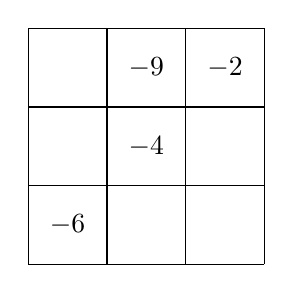
\begin{tikzpicture}
    \draw (0,0) grid (3,3);
    \draw (.5,.5) node {$-6$};
    \draw (1.5,1.5) node {$-4$};
    \draw (1.5,2.5) node {$-9$};
    \draw (2.5,2.5) node {$-2$};
    \end{tikzpicture}
\end{center}

\item Pour l'addition :

\begin{center}
    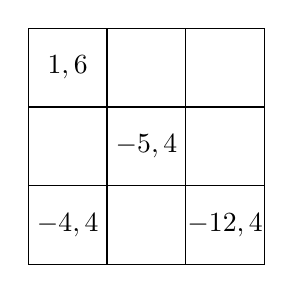
\begin{tikzpicture}
    \draw (0,0) grid (3,3);
    \draw (.5,.5) node {$-4,4$};
    \draw (2.5,.5) node {$-12,4$};
    \draw (1.5,1.5) node {$-5,4$};
    \draw (.5,2.5) node {$1,6$};
    \end{tikzpicture}
\end{center}

\end{enumerate}
\end{exercice}


\begin{exercice}[Signe]
$A$ est le produit de 24 nombres (non nuls) comportant 23 facteurs négatifs.
$B$ est le produit de 13 nombres (non nuls) comportant 11 facteurs négatifs. 
Donne, si c'est possible, le signe de :
\begin{colenumerate}{2}
\item $A \times B$
\item $A \div B$
\item $A -B$ 
\item $A^2$
\item $A + B$
\end{colenumerate}
\end{exercice}



\begin{exercice}[Coup de froid]
Chaque matin de la 1\up{ère} semaine du mois de février, Julie a relevé la température extérieure puis a construit le tableau suivant :

\vspace{.5em}
\renewcommand*\tabularxcolumn[1]{>{\centering\arraybackslash}m{#1}}
\renewcommand{\arraystretch}{1.6}
\begin{ctableau}{\linewidth}{8}
\hline
Jour & Lu & Ma & Me & Je & Ve & Sa & Di \\ \hline
T ($^\circ$C) & $-4$ & $-2$ & $-1$ & $+1$ & 0 & $+2$ & $-3$ \\ \hline
\end{ctableau}

Calcule la moyenne des températures relevées par Julie.
\end{exercice}




\begin{exercice}
Calcule les expressions suivantes en respectant les priorités :

$A = \dfrac{7-7\times 5}{6 \times 2 -5}$ 

$B = (4 -6) \times [5 + (3 -(-2)) \times 2]$

$C = \dfrac{-7 \times (-3) - (-3) \times (-5)}{(12 \div (-3) -2}$
\end{exercice}



\begin{exercice}
Effectue de deux manières différentes les calculs suivants :

$A = (-3) \times (5 -7)$

$B = 5 \times (-4 -3)$

$C = (-7 -2) \times (-3)$

$D = -3 \times ((-4) + (-2))$
\end{exercice}



\begin{exercice}
Calcul d'expressions.
\begin{enumerate}
\item Soit $D = (2\,x+3)^2 + (2\,x+3)(7\,x-2)$. 
Calculer $D$ pour $x = -4$.
\item Soit $E =36-(3\,x+5)^2$. 
Calculer $E$ pour $x = -2$.
\end{enumerate}
\end{exercice}



\begin{exercice}
En détaillant les étapes, calcule :
\begin{enumerate}
\item $A = 3x -7$ pour $x = + 2$ ;
\item $B = -2x -9$ pour $x = -5$ ;
\item $C = x^2 + 2$ pour $x = -1$.
\end{enumerate}
\end{exercice}




\begin{exercice}
Sachant que $a = 5$, $b = -3$ et $c = -10$, calcule les expressions suivantes :

$D = -2\,a$

$E = a -b$

$F = -3\,c + a$

$G = b -a -c$

$H = \dfrac{c}{a} + 2\,b$
\end{exercice}




\begin{exercice}
Calcule $b^2 -4 a\,c$ dans les cas suivants :
\begin{itemize}
    \item 1\up{er} cas : $a = 2$ ; $b = 3$ et $c = 5$.
    \item \up{e} cas : $a = -1$ ; $b = 2$ et $c = 3$.
    \item 3\up{e} cas : $a = 3$ ; $b = -2$ et $c = 2$.
\end{itemize}

\end{exercice}




\begin{exercice}[Conversion]
Aux États-Unis, la température $T$ est mesurée en degrés Fahrenheit. Voici la formule pour convertir une température $T_\text{°F}$ exprimée en degrés Fahrenheit (°F) en une température $T_\text{°C}$ équivalente exprimée en degrés Celsius (°C) :

\[  T_\text{°C} = \dfrac{(T_\text{°F}-32) \times 5}{9}\]

\begin{enumerate} \item À New-York est annoncée une température de 68°F. Convertis cette température en degrés Celsius à l'aide de la formule.
\item Même question pour une température de 23°F.
\item Voici la formule pour convertir une température exprimée en degrés Celsius (°C) en une température équivalente exprimée en degrés Fahrenheit (°F) :

\[ T_\text{°F} = T_\text{°C} \times 1,8 + 32 \]

Recopie puis complète le tableau suivant :

\vspace{.5em}
\renewcommand*\tabularxcolumn[1]{>{\centering\arraybackslash}m{#1}}
\renewcommand{\arraystretch}{1.6}
\begin{ctableau}{\linewidth}{6}
\hline
$T_\text{°C}$ & 0 & 5 & 10 & 15 & 20 \\ \hline
$T_\text{°F}$ & & & & & \\ \hline
\end{ctableau}

\item Place les données du tableau dans un repère similaire à celui ci-dessous.

\begin{center}
    \begin{tikzpicture}
    \draw [quadrillage] (0,0) grid (6,9);
    \axeX{0}{6}{0};
    \draw (2,0) node [below] {10};
    \draw (4,0) node [below] {20};
    \draw (6,0) node [right] {$T_\text{°C}$};
    \axeY{0}{9}{};
    \draw (0,2) node [left] {20};
    \draw (0,4) node [left] {40};
    \draw (0,6) node [left] {60};
    \draw (0,8) node [left] {80};
    \draw (0,9) node [above] {$T_\text{°F}$};
    \end{tikzpicture}
\end{center}

\item  À la vue du graphique, peut-on dire que les deux unités de température sont proportionnelles ? Justifie ta réponse.
\end{enumerate}
\end{exercice}


\end{colonne*exercice}

\connaissances

\QCMautoevaluation{Pour chaque question, plusieurs réponses sont proposées. Déterminer celles qui sont correctes.}

\begin{QCM}
\begin{GroupeQCM}

\begin{exercice}
$-7 \times (-3) =$...
\begin{ChoixQCM}{4}
\item $-10$
\item $-21$
\item 10
\item 21
\end{ChoixQCM}
\begin{corrige}
\reponseQCM{a}
\end{corrige}
\end{exercice}




\begin{exercice}
$(-10) + 15 =$...
\begin{ChoixQCM}{4}
\item $-5$
\item $-150$
\item $5$
\item $25$
\end{ChoixQCM}
\begin{corrige}
\reponseQCM{a}
\end{corrige}
\end{exercice}


\begin{exercice}
$4 \times (-3) =$...
\begin{ChoixQCM}{4}
\item 1
\item $-12$
\item $-7$
\item $12$
\end{ChoixQCM}
\begin{corrige}
\reponseQCM{a}
\end{corrige}
\end{exercice}
 


\begin{exercice}
$-15 \div (-5) =$...
\begin{ChoixQCM}{4}
\item $\dfrac{-15}{-5}$
\item $-3$
\item $15 \div 5$
\item 3
\end{ChoixQCM}
\begin{corrige}
\reponseQCM{a}
\end{corrige}
\end{exercice}


\begin{exercice}
$4 \times (-4) =$...
\begin{ChoixQCM}{4}
\item 0
\item $-8$
\item 16
\item $-16$
\end{ChoixQCM}
\begin{corrige}
\reponseQCM{a}
\end{corrige}
\end{exercice}


\begin{exercice}
$-10 \div 10 =$...
\begin{ChoixQCM}{4}
\item $-0$
\item 1
\item 0
\item $-1$
\end{ChoixQCM}
\begin{corrige}
\reponseQCM{a}
\end{corrige}
\end{exercice}


\begin{exercice}
Le produit de l'opposé de $-6$ par l'opposé de 7 vaut...
\begin{ChoixQCM}{4}
\item 42
\item $-42$
\item $-1$
\item $\dfrac{6}{-7}$
\end{ChoixQCM}
\begin{corrige}
\reponseQCM{a}
\end{corrige}
\end{exercice}


\begin{exercice}
Pour tout nombre relatif $a,$ le nombre $-a$ est...
\begin{ChoixQCM}{4}
\item négatif
\item l'opposé de $a$
\item positif ou négatif suivant le signe de $a$
\item égal à $(-1) \times a$
\end{ChoixQCM}
\begin{corrige}
\reponseQCM{a}
\end{corrige}
\end{exercice}



\begin{exercice}
$-6 + 6 \times (-10) =$...
\begin{ChoixQCM}{4}
\item 0
\item 120
\item 66
\item $-66$
\end{ChoixQCM}
\begin{corrige}
\reponseQCM{a}
\end{corrige}
\end{exercice}


\begin{exercice}
$-12$ est le résultat de...
\begin{ChoixQCM}{4}
\item $3 + 3 \times (-2)$
\item $5 \times (-3) + 3$
\item $(-12 + 5) \div 5$
\item $-8 + 4 \div (2 -3)$
\end{ChoixQCM}
\begin{corrige}
\reponseQCM{a}
\end{corrige}
\end{exercice}




\begin{exercice}
Pour tous nombres relatifs $u$ et $v$, le produit $-u \times v \times u \times v$ est...
\begin{ChoixQCM}{4}
\item nul
\item positif
\item négatif
\item de signe  impossible à déterminer
\end{ChoixQCM}
\begin{corrige}
\reponseQCM{a}
\end{corrige}
\end{exercice}






\begin{exercice}
Le produit de 108 facteurs égaux à $-1$ est égal à...
\begin{ChoixQCM}{4}
\item $-108$
\item 0
\item $-1$
\item 1
\end{ChoixQCM}
\begin{corrige}
\reponseQCM{a}
\end{corrige}
\end{exercice}
\end{GroupeQCM}
\end{QCM}


\begin{QCM}
\begin{GroupeQCM}


\begin{exercice}
$x$ est le relatif tel que $x \times (-3) = -10$ donc...
\begin{ChoixQCM}{4}
\item $x = -7$
\item $x = 3,33$
\item $x=\dfrac{10}{3}$
\item $-\dfrac{10}{3}$
\end{ChoixQCM}
\begin{corrige}
\reponseQCM{a}
\end{corrige}
\end{exercice}



\begin{exercice}
$a$ est un nombre négatif donc...
\begin{ChoixQCM}{4}
\item $a^2$ est négatif
\item $-a^2$ est négatif
\item $(-a)^2$ est négatif
\item $\dfrac{a}{-a}=0$
\end{ChoixQCM}
\begin{corrige}
\reponseQCM{a}
\end{corrige}
\end{exercice}


\begin{exercice}
Dans un produit de 90 facteurs...
\begin{ChoixQCM}{4}
\item un facteur est égal à 0 donc ce produit est égal à 0
\item il y a deux  facteurs positifs donc ce produit est positif
\item il n'y a que des facteurs négatifs donc ce produit est négatif
\item Il y a trois facteurs négatifs donc ce produit est négatif
\end{ChoixQCM}
\begin{corrige}
\reponseQCM{a}
\end{corrige}
\end{exercice}


\end{GroupeQCM}
\end{QCM}


\TravauxPratiques
\begin{TP}[Le bon produit]

\partie{La construction du jeu}

Avec du papier épais ou du carton, fabriquez  66 cartes à jouer.

Au stylo bleu, fabriquez les 38 cartes « facteur » :
\begin{itemize}
\item deux portent le nombre 0 ;
\item trois exemplaires pour chacun des nombres : $-9$ ; $-6$ ; $-4$ ; $-3$ ; $-2$ ; $-1$ ; 1 ; 2 ; 3 ; 4 ; 6 et 9.
\end{itemize}

Remarque : Soulignez les 6 et les 9 pour éviter de les confondre.

Au stylo rouge, fabriquez les 28 cartes « produit » : 
\begin{itemize}
\item deux portent le nombre 0 ;
\item les autres sont toutes différentes et portent les nombres : $-54$ ; $-36$ ; $-27$ ; $-24$ ; $-18$ ; $-16$ ; $-12$ ; $-9$ ; $-8$ ; 6 ; $-4$ ; $-3$ ; $-2$ ; 2 ; 3 ; 4 ; 6 ; 8 ; 9 ; 12 ; 16 ; 18 ; 24 ; 27 ; 36 et 54.
\end{itemize}

\partie{Les règles du jeu}

Chaque joueur reçoit six cartes « facteur » puis pioche une carte « produit ». Celui qui a le plus grand nombre joue en premier (en cas d'égalité, les joueurs ex-aequo piochent une deuxième carte « produit »). On tourne ensuite dans le sens des aiguilles d'une montre.

Les cartes « produit » piochées sont posées face visible. On complète de façon à en avoir 10 en tout sur la table.

Le joueur dont c'est le tour pioche une carte « produit » et la pose sur la table avec les autres. 

Si, avec deux de ses cartes facteurs, il peut obtenir un des produits visibles, il écarte les trois cartes (les deux cartes « facteur » et la carte « produit »).
S'il ne peut pas, il pioche deux cartes « facteur » et regarde à nouveau s'il peut obtenir un produit.

S'il propose une combinaison et qu'il a fait une erreur de calcul, il pioche également deux cartes « facteur ».

C'est alors au tour du joueur suivant.

Lorsqu'un joueur a écarté toutes ses cartes « facteur », il a gagné.

\end{TP}

%%%%%%%%%%%%%%%%%%%%%%%%%%%%%%%%%%%
%%%%%%%%%%%%%%%%%%%%%%%%%%%%%%%%%%%


\begin{TP}[Expressions littérales]

\partie{Résolution d'énigmes}

Dans chaque cas, retrouvez les valeurs de chacune des inconnues pour que l'égalité soit vérifiée sachant qu'elles sont données dans le désordre.

Exemple : Pour le problème :

\renewcommand*\tabularxcolumn[1]{>{\centering\arraybackslash}m{#1}}
\renewcommand{\arraystretch}{1.6}
\begin{Ctableau}{\linewidth}{6}{c}
\hline
$a(b -c) -de = -5$ & 4 & $-1$ & $-3$ & $-2$ & 1 \\ \hline
\end{Ctableau}

Une solution est : $a = -3$ ; $b = 1$ ; $c = -2$ ; $d = 4$ et $e = -1$. En effet :

$-3 \times (1 -(-2)) -4 \times (-1) = -9 + 4 = -5$.

\vspace{1em}

\textbf{Niveau 1 : trois inconnues}

\vspace{1em}

\renewcommand*\tabularxcolumn[1]{>{\centering\arraybackslash}m{#1}}
%\renewcommand{\arraystretch}{1.6}
\begin{Ctableau}{\linewidth}{4}{c}
\hline
$a + b -c = 3$ & $-2$ & 4 & $-3$ \\ \hline
$a + bc = 1$ & $-1$ & 3 & 4 \\ \hline
$a -(b -c) = 1$ & $-5$ & 2 & 8 \\ \hline
$\dfrac{a}{-b+c} = -1,5$ & 3 & 1 & $-3$ \\ \hline
$a+\dfrac{b}{c} = 3$ & $-1$ & 2 & 5 \\ \hline
\end{Ctableau}


\vspace{1em}

\textbf{Niveau 2 : quatre inconnues}

\vspace{1em}

\renewcommand*\tabularxcolumn[1]{>{\centering\arraybackslash}m{#1}}
%\renewcommand{\arraystretch}{1.6}
\begin{Ctableau}{\linewidth}{5}{c}
\hline
$(a + b)(c + d) = -60$ & $-9$ & $-4$ & $-3$ & 9 \\ \hline
$\dfrac{a-b}{c+d} = 3$ & $-9$ & $-3$ & 9 & 9 \\ \hline
$a(b -c) -d = 17$ & 4 & $-5$ & 7 & $-8$ \\ \hline
$ab -cd = 1$ & $-3$ & $-5$ & 5 & 8 \\ \hline
$a -\dfrac{b}{c} -d = -7$ & $-6$ & $-10$ & 5 & 3 \\ \hline
\end{Ctableau}

\vspace{1em}

\textbf{Niveau 3 : cinq inconnues}

\vspace{1em}

\renewcommand*\tabularxcolumn[1]{>{\centering\arraybackslash}m{#1}}
%\renewcommand{\arraystretch}{1.6}
\begin{Ctableau}{\linewidth}{6}{c}
\hline
$a(b + c) -de = 19$ &
$-1$ &
3 &
2 &
5 &
$-6$ \\ \hline
$\dfrac{a}{b+c}- \dfrac{d}{e} = -1$ & $-1$ & 3 & 8 & 2 & 4 \\ \hline
$a(b + c) -a(d -e) = 1$ & 2 & 4 & $-1$ & $-2$ & 3 \\ \hline
\end{Ctableau}



\partie{\'A vous de faire les énigmes}

Maintenant, construisez des énigmes sur le modèle précédent : deux de niveau 1, deux de niveau 2 et une de niveau 3.

Les énigmes seront ensuite rassemblées au tableau et chaque groupe devra essayer d'en résoudre le plus grand nombre possible.


\end{TP}

%%%%%%%%%%%%%%%%%%%%%%%%%%%%%%%%%%%
%%%%%%%%%%%%%%%%%%%%%%%%%%%%%%%%%%%

\recreation % avec R majuscule pour saut de page
\begin{enigme}[Des signes...]
\begin{enumerate}
    \item $a$, $b$ et $c$ sont trois nombres relatifs dont le produit est négatif et $b$ est le double de $a$.
    
    Quel est le signe de $c$ ?
    \item $x$, $y$ et $z$ sont trois nombres relatifs tels que :
		$x \times y$ et $x \times z$ ont le même signe ;
		$y$ et $y \times z$ ont le même signe ;
		$y$ et $x \times y \times z$ ont des signes différents.
		
	Quels sont les signes de $x$, $y$ et $z$ ?
	\item Pour quelles valeurs de $m$, le produit de $m$ par $m -1$ est-il négatif ?
	\item Donne le signe de $x -1$ en fonction des valeurs de $x$.
Étudie le signe du produit $x(x -1)(x -2)$ en fonction des valeurs de $x$.
\end{enumerate}
\end{enigme}

\vspace{2em}

\begin{enigme}[La danse des signes]
Certains nombres relatifs ont perdu leur signe et il peut manquer des signes d'opérations ! À toi de les retrouver !

$(-2) \times (... 3) -(-8) \times (... 2) = 22$ ;

$(-2) \times (... 3) -(-8) \div (... 2) = 2$ ;

$(-2) ... (... 3) -(-8) \times (... 2 ... 4) = -10$.
\end{enigme}


\vspace{2em}

\begin{enigme}[Que de signes !]
Détermine le signe du produit suivant :

$(-343) \times (-344) \times (-345) \times ... \times (-999)$.
\end{enigme}



\vspace{2em}

\begin{enigme}[Le compte est bon]
Avec les nombres proposés, retrouve les résultats annoncés !

Tu ne peux utiliser chaque nombre qu'une seule fois. Toutes les opérations sont autorisées.

Avec $-3$ ; $-5$ ; 25 ; $-100$ et 7, trouve $-650$ !

Avec $-7$ ; $-25$ ; 10 ; $-8$ et $-75$, trouve 730 !
\end{enigme}


\vspace{2em}

\begin{enigme}[Qui suis-je ?]
Ce nombre est très bizarre : que je le multiplie par $-2$ ou par $-7$, j'obtiens le même résultat ! Quel est ce nombre ?

Quand je me multiplie par moi-même, cela donne mon opposé ! Qui suis-je ?
\end{enigme}



\vspace{2em}

\begin{enigme}[Des signes, toujours des signes...]
$a$ et $b$ sont des nombres relatifs. Étudie leurs signes dans chacun des cas suivants :
\begin{itemize}
    \item $a + b$ est un nombre négatif et $a \times b$ est un nombre positif ;
    \item $a + b$ et $a \times b$ sont des nombres négatifs.
\end{itemize}
\end{enigme}


\vspace{2em}

\begin{enigme}[Les nombres négatifs dans l'histoire]
Les nombres négatifs font aujourd'hui partie de notre environnement. Nous les considérons comme des nombres à part entière.

Pourtant, leur introduction dans les mathématiques fut lente, difficile et maintes fois remise en cause. Ils naissent à travers les calculs de gains et de dettes. On attribue aux Chinois les premières utilisations de quantités négatives au premier siècle de notre ère.

\vspace{1em}


Voici ce que disait, en 1803, le mathématicien et ingénieur Lazare Carnot (1753 - 1823) à leur propos :

{\em « Pour obtenir réellement une quantité négative isolée, il faudrait retrancher une quantité effective de zéro, ôter quelque chose de rien : opération impossible. Comment donc concevoir une quantité négative isolée ? ».}

\vspace{1em}

Voici deux autres citations de mathématiciens :

\vspace{1em}

Pascal (1623 - 1662), dans ses « Pensées » :

{\em « Trop de vérité nous étonne ; j’en sais qui ne peuvent comprendre que, qui de zéro ôte 4, reste zéro. ».}

\begin{center}
    \includegraphics[width=2cm]{pascal}
    
\hfill {\footnotesize (Image : Pascal, source Wikipédia)}
\end{center}


\vspace{1em}

Arnauld (un ami de Pascal), à propos de l’égalité $\dfrac{-1}{1}=\dfrac{1}{-1}$ :

{\em « Comment un nombre plus petit pourrait-il être à un plus grand comme un plus grand à un plus petit ? ».}

\begin{enumerate}
    \item Explique ces phrases et commente-les.
    \item Et que penser de la réflexion suivante de Wallis (1616 - 1703) ?
    
{\em « a étant un nombre positif, le quotient  est infini. Comme  est plus grand, le dénominateur étant plus petit, il est plus grand que l’infini tout en étant inférieur à zéro car le résultat est négatif. »}
\end{enumerate}

\end{enigme} 

%%%%%%%%%%%%%%%%%%%%%%%%%%%%%%%%%%%%%%%%%%%%%%%%%
%%%%%%%%%%%%%%%%%%%%%%%%%%%%%%%%%%%%%%%%%%%%%%%%%


